% ======================================================================
%  Compile with pdflatex.
% ======================================================================
\documentclass{sig-alternate}
\usepackage{jeffe,graphicx,hyperref}
\usepackage[obey]{fixacm}

%-----------------------------------------------------------------------
%  These packages are purely cosmetic.
%  Just comment them out if they don't work for you.
%-----------------------------------------------------------------------
%\usepackage{txfonts}
\usepackage{microtype}
\usepackage[charter]{mathdesign}
\def\sfdefault{fvs}
\def\ttdefault{fvm}
\usepackage[mathcal]{euscript}
\usepackage{stmaryrd}

\def\note#1{\EMPH{\color{red} #1}}

\clubpenalty 5000
\widowpenalty 5000

%-----------------------------------------------------------------------
%  Local definitions
%-----------------------------------------------------------------------
\makeatletter % less nice replacements for stmaryrd characters
\@ifundefined{shortrightarrow}{\let\shortrightarrow\rightarrow}{}
\@ifundefined{shortleftarrow}{\let\shortleftarrow\leftarrow}{}
\@ifundefined{shortuparrow}{\let\shortuparrow\uparrow}{}
\@ifundefined{shortdownarrow}{\let\shortdownarrow\downarrow}{}
\makeatother

\def\arc#1#2{#1\mathord\shortrightarrow#2}
\def\cra#1#2{#1\mathord\shortleftarrow#2}
\def\fence#1#2{#1\mathord\shortuparrow#2}
\def\ecnef#1#2{#1\mathord\shortdownarrow#2}
\def\head{\operatorname{head}}
\def\tail{\operatorname{tail}}
\def\lsh{\operatorname{left}}
\def\rsh{\operatorname{right}}
\def\rev{\operatorname{rev}}
\def\head{\emph{head}}
\def\tail{\emph{tail}}
\def\lsh{\emph{left}}
\def\rsh{\emph{right}}
\def\rev{\emph{rev}}
\def\Z{\mathbb{Z}}
\def\N{\mathbb{N}}
\def\Real{\mathbb{R}}
\def\Q{\mathbb{Q}}

\def\dvec#1{\vec{#1}\,^*}       % dual dart
\def\bdry{\mathord{\partial\!}} % mathdesign puts extra space after \partial
%\def\bdry{\partial}
\def\opt#1{#1_{\emph{OPT}}}
\def\Cmax{U}
\def\Csum{C}
\def\Cmin{c_{\min}}

\def\fakeparagraph#1{\medskip\noindent\textbf{#1}~}

\newtheorem{theorem}{Theorem}[section]
\newtheorem{corollary}[theorem]{Corollary}
\newtheorem{lemma}[theorem]{Lemma}


% ----------------------------------------------------------------------
\begin{document}

\conferenceinfo{SCG'09,} {June 8--10, 2009, Aarhus, Denmark.} 
\CopyrightYear{2009}
\crdata{978-1-60558-501-7/09/06} 

\title{Minimum Cuts and Shortest Homologous Cycles%
	\huge\thanks{Research partially supported by NSF grant DMS-0528086.}}

\author{
    Erin W. Chambers
    \\[0.5ex]
	\affaddr{Department of Computer Science and Mathematics}\\
	\affaddr{Saint Louis University}\\
	\email{\url{echambe5@slu.edu}}
\alignauthor
    \and
	Jeff Erickson\\[0.5ex]
	\affaddr{Department of Computer Science}\\
    \affaddr{University of Illinois, Urbana-Champaign}\\
	\email{\url{jeffe@cs.uiuc.edu}}
\alignauthor
	Amir Nayyeri\\[0.5ex]
	\affaddr{Department of Computer Science}\\
    \affaddr{University of Illinois, Urbana-Champaign}\\
	\email{\url{nayyeri2@illinois.edu}}
}
\maketitle

\begin{abstract}
We describe the first algorithms to compute minimum cuts in surface-embedded graphs in near-linear time.  Given an undirected graph embedded on an orientable surface of genus~$g$, with two specified vertices $s$ and $t$, our algorithm computes a minimum $(s,t)$-cut in $g^{O(g)} n\log n$ time.  Except for the special case of planar graphs, for which $O(n\log n)$-time algorithms have been known for more than 20 years, the best previous time bounds for finding minimum cuts in embedded graphs follow from algorithms for general sparse graphs.  A slight generalization of our minimum-cut algorithm computes a minimum-cost subgraph in every $\Z_2$-homology class.  We also prove that finding a minimum-cost subgraph homologous to a single input cycle is {NP}-hard.
\end{abstract}


\category{F.2.2}
{Analysis of Algorithms and Problem Complexity}
{Nonnumerical Algorithms and Problems}
[Computations on discrete structures]
%
\category{G.2.2}
{Discrete Mathematics}
{Graph theory}
[Graph algorithms]

\terms{Algorithms, Performance}

\keywords{computational topology, topological graph theory}

\bigskip
\begin{rightquote}{0.4}
Bin \"ol\c c, bir kes.\\{}
[Measure a thousand times, cut once.]
\quotee{Turkish proverb\qquad\qquad\qquad~}
\end{rightquote}


% ----------------------------------------------------------------------------

\section{Introduction}

Planar graphs have been a natural focus of study for algorithms research for decades, both because they accurately model many real-world networks, and because they often admit simpler and/or more efficient algorithms for many problems than general graphs.  Most planar-graph algorithms either apply immediately or have been quickly generalized to larger families of graphs, such as graphs of higher genus, graphs with forbidden minors, or graphs with small separators.  Examples include minimum spanning trees \cite{p-omst-99, m-tltam-04}; single-source and multiple-source shortest paths \cite{cc-msspg-07, fr-pgnwe-06, hkrs-fspap-97, k-msspp-05, kmw-spdpg-09, lrt-gnd-79, tm-spltm-09}; graph and subgraph isomorphism \cite{g-itegd-00, hw-ltaip-74, m-itgbg-80, e-sipgr-99, e-dtmcg-00}; and approximation algorithms for the traveling salesman problem, Steiner trees, and other NP-hard problems~\cite{bdt-ptass-08, bkk-ptass-07, bkk-stpg-07, dhm-aacd-07, e-dtmcg-00}.

The classical minimum cut problem and its dual, the maximum flow problem, are stark exceptions to this general pattern.  Flows and cuts were introduced in the 1950s as tools for studying transportation networks, which are naturally modeled as planar graphs \cite{hr-fmern-55}.  Ford and Fulkerson's seminal paper \cite{ff-mfn-56} includes an algorithm to compute maximum flows in planar networks where the source and target lie on the same face.  A long series of results eventually led to planar minimum-cut algorithms that run in $O(n\log n)$ time, first for undirected graphs \cite{r-mstcp-83, hj-oamfu-85, f-faspp-87} and later for directed
graphs \cite{jk-mcdpn-92, hkrs-fspap-97}.  Strangely, however, almost nothing is known about computing flows and cuts in generalizations of planar graphs.  Even for graphs embedded on the torus, the fastest known minimum-cut algorithms have no better performance than for general sparse graphs.

This paper describes the first algorithm to compute minimum cuts in surface-embedded graphs of fixed genus in near-linear time.  Before describing our results in detail, we first review several related results; technical terms are defined in Section \ref{S:background}.

%
%\note{Erin: Reviewers commented that we needed to formally define s,t cuts in the intro.  I think we might want it in the background section instead of here, but I put it just below for now.  Feel free to adjust.}

\fakeparagraph{Planar minimum cuts.}
Recall that for any two vertices $s$ and~$t$ in a graph $G$, an \EMPH{$(s,t)$-cut} is a subset of the edges of $G$ that intersects every path from $s$ to $t$.  A \emph{minimum} $(s,t)$-cut is an $(s,t)$-cut of minimum size, or minimum total weight if the edges of $G$ are weighted.

Itai and Shiloach \cite{is-mfpn-79} observed that the minimum $(s,t)$-cut in a planar graph~$G$ is dual to the minimum-cost cycle that separates faces $s^*$ and $t^*$ in the dual graph $G^*$.  They also observed that this separating cycle intersects any shortest path from a vertex of $s^*$ to a vertex of $t^*$ exactly once.  Thus, one can compute the minimum cut by cutting the dual graph $G^*$ along a shortest path~$\pi$ from $s^*$ to~$t^*$; duplicating every vertex and edge of $\pi$; and then computing, for each vertex $u$ of $\pi$, the shortest path between the two copies of $u$ in the resulting planar graph.  Applying Dijkstra's shortest-path algorithm at each vertex of~$\pi$ immediately yields a running time of $O(n^2\log n)$.

Reif \cite{r-mstcp-83} improved the running time of this algorithm to $O(n\log^2 n)$ using a divide-and-conquer strategy.  Reif's algorithm was extended by Hassin and Johnson to compute the actual maximum flow in $O(n\log n)$ additional time, using a carefully structured dual shortest-path computation \cite{hj-oamfu-85}.  Frederickson~\cite{f-faspp-87} subsequently improved the running time of Reif's algorithm to $O(n\log n)$ using a balanced separator decomposition to speed up the shortest-path computations.  Janiga and Koubek~\cite{jk-mcdpn-92} adapted Reif's $O(n\log^2 n)$-time algorithm to directed planar graphs.  Henzinger \etal~\cite{hkrs-fspap-97} generalized Frederickson's technique to obtain an $O(n)$-time planar shortest-path algorithm; using this algorithm in place of Dijkstra's algorithm improves the running times of both Reif's and Janiga and Koubek's algorithms to $O(n\log n)$.  The same improvement can also be obtained using more recent multiple-source shortest path algorithms by Klein~\cite{k-msspp-05} and Cabello and Chambers \cite{cc-msspg-07}.

Minimum cuts in directed planar graphs can also be obtained in $O(n\log n)$ time using the planar maximum-flow algorithms of Weihe \cite{w-mstfp-97} (if the graph satisfies certain connectivity restrictions) and Borradaile and Klein \cite{b-epnfc-08, bk-tamfd-06, bk-amfdp-09}.

\fakeparagraph{Generalizations of planar graphs.}
Surprisingly little is known about the complexity of computing maximum flows or minimum cuts in generalizations of planar graphs.  In particular, we know of no algorithm to compute minimum cuts in non-planar graphs that does not first compute a maximum flow.

By combining a technique of Miller and Naor \cite{mn-fpgms-95} with the planar directed flow algorithm of Borradaile and Klein \cite{b-epnfc-08, bk-tamfd-06, bk-amfdp-09}, one can compute maximum (single-commodity) flows in a planar graph with $k$ sources and sinks in $O(k^2 n\log n)$ time.  A recent algorithm of Hochstein and Weihe \cite{hw-mstfkc-07} computes a maximum flow in a planar graph with $k$ additional edges in $O(k^3n\log n)$ time, using a clever simulation of Goldberg and Tarjan's push-relabel algorithm~\cite{gt-namfp-88}.

To our knowledge, the only prior max-flow algorithm that applies to graphs of positive genus, but not to arbitrary sparse graphs, is an algorithm of Imai and Iwano \cite{ii-espap-90} that computes minimum-cost flows in graphs with small balanced separators, using a combination of nested dissection \cite{lrt-gnd-79, pr-fepss-93}, interior-point methods~\cite{v-slpfm-89}, and fast matrix multiplication.  Their algorithm can be adapted to compute maximum flows (and therefore minimum cuts) in any graph of constant genus in time $O(n^{1.595}\log C)$, where $C$ is the sum of the capacities.  However, this is slower than more recent and more general algorithms \cite{gr-bfdb-98}.

Euler's formula implies that a simple $n$-vertex graph embedded on a surface of genus $O(n)$ has at most $O(n)$ edges.  The fastest known combinatorial maximum-flow algorithms for sparse graphs, due to Sleator and Tarjan~\cite{st-dsdt-83} and Goldberg and Tarjan~\cite{gt-namfp-88}, run in time $O(n^2\log n)$.  The fastest algorithm known for integer capacities, due to Goldberg and Rao \cite{gr-bfdb-98}, runs in time $O(n^{3/2}\log n\log U)$, where $U$ is an upper bound on the edge capacities.  These are also the fastest algorithms previously known for computing maximum flows or minimum cuts in graphs of any positive genus.

For further background on maximum flows, minimum cuts, and related problems, we refer the reader to monographs by Ahuja \etal\ \cite{amo-nftaa-93} and Schrijver \cite{s-cape-03}.

\fakeparagraph{Short interesting cycles.}
Many different problems, such as finding approximate traveling salesman tours  \cite{dhm-aacd-07} and Steiner trees~\cite{bdt-ptass-08} in surface embedded graphs, embedding high-genus graphs into the plane with low distortion \cite{is-pebgg-07} or with few crossings \cite{kr-ccnlt-07}, and feature detection and simplification in meshes \cite{gw-tnr-01,dlsc-cgaht-08}, require algorithms to find short but topologically nontrivial cycles.

Thomassen described the first efficient algorithm to find the shortest non-contractible or non-separating cycle \cite{t-egnsn-90, mt-gos-01}.  After many intermediate improvements \cite{c-mdpg-06, cm-fsnsn-07, eh-ocsd-04, k-csnco-06}, Cabello and Chambers~\cite{cc-msspg-07} described the fastest algorithm currently known for this problem, which runs in $O(g^3 n \log n)$ time.  Splitting cycles are non-contractible and separating; finding the shortest such cycle is {NP}-hard, although there is an $O(n \log n)$-time algorithm for graphs of any fixed genus \cite{ccelw-scsih-06, ccelw-scsih-08}.  Colin de Verdi\`ere and Erickson~\cite{ce-tspcs-06} prove that the shortest path or cycle in a given homotopy class can be computed in polynomial time, improving earlier results of Colin de Verdi\`ere and Lazarus \cite{c-rcds-03, cl-oslos-05, cl-opdsh-07}.  Erickson and Whittlesey describe a greedy algorithm to find a minimum-length set of cycles that generate the first homology group of a surface \cite{ew-gohhg-05}.

Several practical heuristics have been developed for finding short cycles that work well in practice, although they have no theoretical guarantees.  For example, Guskov and Wood \cite{gw-tnr-01} describe an algorithm to find and remove intersecting pairs of short non-contractible cycles (`topological noise') from surface meshes.  Zomorodian and Carlsson \cite{zc-lh-07} define the \emph{localized} homology of an arbitrary topological case with respect to a subspace covering; they also describe algorithms to compute localized homology generators of simplicial complexes using persistent homology; however, they do not describe how to compute covers that would lead to cycles of minimum size.  Chen and Friedman \cite{cf-qhc2-07, cf-qhc-08} describe a polynomial-time algorithm to compute a cycle of minimum \emph{radius} in a given homology class, in an arbitrary edge-weighted simplicial complex; however, the length of this cycle could be arbitrarily longer than optimal.

Dey \etal~\cite{dls-chtl-07, dlsc-cgaht-08} describe algorithms to find short \emph{handle} and \emph{tunnel} cycles in surface meshes embedded in $\Real^3$.  Any embedded surface subdivides $\Real^3$ into an inner handlebody $I$ and an outer handlebody $O$; handle cycles are null-homologous in $I$, while tunnel cycles are null-homologous in~$O$.  The algorithm of Dey \etal\ finds $g$ short handle cycles and $g$ short tunnel cycles that collectively generate the first homology group of the input surface.  Their algorithm uses several heuristics to reduce the length of the output cycles, in part because no algorithm is known to find the shortest cycle in a given homology class.

\fakeparagraph{New Results.}
The input to our algorithm is an undirected edge-weighted graph~$G$ embedded on an orientable surface of genus~$g$.  Given vertices $s$ and $t$, our algorithm computes a minimum-weight $(s,t)$-cut in $g^{O(g)}n\log n$ time.  For any fixed positive genus, this improves the best previous time bound by a factor of $\min\set{n, \sqrt{n}\log C}$.

Our minimum-cut algorithm is a special case of a more general algorithm to compute a minimum-cost \emph{subgraph} in a given $\Z_2$-homology class.  Even when the homology class is specified by a simple cycle, the output representative may be the union of several cycles; see Figure \ref{F:homology2}.  For surfaces with genus $g$ and $b$ boundary components, our algorithm runs in $(g+b)^{O(g+b)}n\log n$ time.  We also show that this more general problem is strongly NP-hard, even if the input homology class is specified by a simple cycle; thus, the exponential dependence on the topology of the surface is unavoidable unless {P}={NP}.  We are not aware of any previous algorithmic results for our more general problem.

Of course, the original minimum-cut problem is not NP-hard!  We conjecture that minimum cuts can be computed in time $O(g^c n\log n)$ for some small constant $c$.

%\note{Reviewer 2 says: "It wouldn't hurt expliciting that you don't know
%whether your min-cut problem is NP-hard."}

%\note{Erin: Not sure I agree with reviewer 2, so I didn't add that.}

%\note{Jeff: Of course it isn't NP-hard!}

In a companion paper~\cite{cen-hfcc-09}, we describe algorithms to compute a maximum flow in surface embedded graphs, using very different techniques from this paper.  Specifically, given an undirected graph embedded on an orientable surface of genus~$g$, with two specified vertices $s$ and $t$, we can compute a maximum $(s,t)$-flow in $O(g^7 n\log^2 n\log^2 C)$ time for integer capacities that sum to $C$, or in $(g\log n)^{O(g)} n$ time for real capacities.  Our key insight is that it suffices to optimize the relative homology class of the flow, rather than directly optimizing the flow itself.

% ----------------------------------------------------------------------------

% ----------------------------------------------------------------------------
\section{Dramatis Personae}
\label{S:background}

%\note{Comments by reviewers for this section are very mixed.  Reviewer 1 felt very strongly that we spend too much time on background, while 2 and 3 think the background/exposition here is nice.  I (Erin) like it as is, and think the background is a good idea since this much homology might be new to the typical SOCG reader, but maybe I'm mistaken.}

%\note{Jeff: The background is partly here for the benefit of (a) readers of the other paper, who need to see the differences in the definitions; (b) }

We begin by recalling several useful definitions related to graphs
embedded on surfaces.  For more comprehensive treatments, we refer
the interested reader to Gross and Tucker \cite{gt-tgt-01} and Mohar
and Thomassen~\cite{mt-gos-01} for topological graph theory, and to
Hatcher~\cite{h-at-01} and Stillwell~\cite{s-ctcgt-93} for topology.

%\note{This is \emph{way} more than we really need, but better to
%have too much than too little at this point.  Do we really need to
%define darts?  Rotation systems?  Left and right shore?
%Combinatorial surfaces?  Path homotopy?  Covering spaces?
%Cohomology?  We do need boundaries for the minimum-cut algorithm.}

%\note{Erin: I think we need rotation systems, combinatorial
%surfaces, homotopy and homology, and cohomology (based on current
%section 3).  We don't seem to need darts or covering spaces at all,
%so I commented those out.  Feel free to re-add if necessary.}


\subsection{Surfaces and Curves}

A \EMPH{surface} (more formally, a \emph{2-manifold}) $\Sigma$ is a
compact topological space in which every point has an open
neighborhood homeomorphic to either the plane $\Real^2$ or a closed
halfplane $\set{(x,y)\in \Real^2\mid x\ge 0}$.  The points with
halfplane neighborhoods comprise the \EMPH{boundary} of the surface;
every connected component of the boundary is homeomorphic to a
circle.  A surface is \emph{non-orientable} if it contains a
subset homeomorphic to the \Mobius\ band, and \emph{orientable}
otherwise.

A \EMPH{path} in a surface $\Sigma$ is a continuous function $p\colon [0,1]\to\Sigma$.  A \EMPH{loop} is a path whose endpoints $p(0)$ and $p(1)$ coincide; we refer to this common endpoint as the \EMPH{basepoint} of the loop.  An \EMPH{arc} is a path whose endpoints  lie on the boundary of $\Sigma$.  A \EMPH{cycle} is a continuous function $\gamma\colon S^1\to\Sigma$.  We refer to paths, loops, arcs, and cycles as \EMPH{curves}.  We will usually not distinguish between a path/cycle and its image in $\Sigma$.  A curve is \EMPH{simple} if the function that defines it is injective, except for the basepoint in the case of loops.  The \EMPH{reversal $\overline{p}$} of a path $p$ is defined by setting $\overline{p}(t) = p(1-t)$.  The \EMPH{concatenation $p \cdot q$} of two paths $p$ and $q$ with $p(1) = q(0)$ is the path created by setting $(p\cdot q)(t) = p(2t)$ for all $t \le 1/2$ and $(p\cdot q)(t) = q(2t-1)$ for all $t \ge 1/2$.

The \EMPH{genus} of a surface $\Sigma$ is the maximum number of simple, disjoint, non-separating cycles $\gamma_1, \gamma_2, \dots, \gamma_g$; that is, $\gamma_i\cap\gamma_j = \varnothing$ for all $i$ and $j$, and the surface $\Sigma\setminus(\gamma_1\cup\cdots\cup\gamma_g)$ is connected.  This paper will consider only compact, connected, orientable surfaces.  Up to homeomorphism, there is exactly one such surface with any non-negative genus $g$ and any non-negative number of boundaries $b$.

%The line below is commented out as per Reviewer 2's comment, since we haven't defined n yet.
%We will assume that $g+b = o(n)$, since we improve existing results only when $g$ and $b$ are small.

\subsection{Graph Embeddings}

%Let $G = (V,E)$ be an undirected graph.  We define an associated directed graph $\vec{G} = (V, \vec{E})$ by replacing each undirected edge in $E$ with an antisymmetric pair of directed edges.  The graphs $G$ and $\vec{G}$ are represented by the same adjacency matrix.  We refer to the directed edges in $\vec{E}$ as \EMPH{darts}.  Each dart connects two (possibly equal) vertices, called its \EMPH{tail} and its \EMPH{head}; we say that the dart \EMPH{leaves} its tail and \EMPH{enters} its head.%  Each dart~$\vec{e}$ has a unique \EMPH{reversal}, denoted $\rev(\vec{e})$ and defined by swapping its endpoints: $\head(\rev(\vec{e})) = \tail(\vec{e})$ and $\tail(\rev(\vec{e})) = \head(\vec{e})$.  We will often write \EMPH{$\arc{u}{v}$} to denote a dart with tail $u$ and head $v$; thus, $\rev(\arc{u}{v}) = \arc{v}{u}$.

An \EMPH{embedding} of an undirected graph~$G$ on a surface $\Sigma$ consists of a mapping of vertices of $G$ to distinct points in~$\Sigma$ and a collection of mappings from edges of $G$ to simple paths in $\Sigma$ that intersect only at common endpoints.  A~\EMPH{face} of an embedding is a maximal connected subset of~$\Sigma$ that does not intersect the image of any edge or vertex.  An embedding is \EMPH{cellular} (or \emph{2-cell} \cite{mt-gos-01}) if every face is an open topological disk; in particular, in any cellular embedding, the boundary of $\Sigma$ is covered by edges of $G$.

% Any cellular embedding can be represented combinatorially by a \EMPH{rotation system}, which encodes the cyclic ordering of edges incident to each vertex.
%\note{Amir: Do we need this paragraph?}
%It is useful to view weighed graphs as continuous metric spaces, so
%that distances and shortest paths between points in the interior of
%edges are well-defined.  Specifically, each edge with weight~$\ell$
%is isometric to the real interval $[0,\ell]$.  We do \emph{not}
%assume that the edge weights obey the triangle inequality; in
%particular, the shortest path between two points on an edge is not
%necessarily contained in that edge.

Suppose $G$ is a simple $n$-vertex graph cellularly embedded on an orientable surface of genus $g$ with~$b$ boundaries.  Euler's formula $\abs{V}-\abs{E}+\abs{F} = 2-2g-b$ implies that $G$ has at most $3n-6+6g+3b$ edges and at most $2n-4+4g+2b$ faces, with equality if every face of the embedding and every boundary cycle is a triangle.  Thus, the overall complexity of an embedding of an $n$-vertex graph is $O(n+g+b) = O(n)$.

%\note{Omit this paragraph?}
%Every dart in an embedded graph $G$ separates two (possibly equal) faces, called the \EMPH{left shore} and \EMPH{right shore}.  We say that a dart $\vec{e}$ \EMPH{winds counterclockwise} around $\lsh(\vec{e})$ and \EMPH{winds clockwise} around $\rsh(\vec{e})$. Reversing the dart swaps these two faces: $\lsh(\rev(\vec{e})) = \rsh(\vec{e})$ and $\rsh(\rev(\vec{e})) = \lsh(\vec{e})$.  We will sometimes write \EMPH{$\fence{f}{g}$} to denote a dart whose left shore is $f$ and whose right shore is $g$; thus, $\rev(\fence{f}{g}) = \fence{g}{f}$.  See Figure \ref{F:primaldual}.

%A cellular embedding can be alternately represented combinatorially by a permutation $\varpi$ of its darts that describe its \EMPH{facial cycles} (or \emph{circuits}).  Specifically, $\varpi(\vec{e})$ is the dart that appears immediately after $\vec{e}$ in the clockwise ordering of darts that wind clockwise around $\lsh(\vec{e})$.  The rotation system of a cellular embedding determines its facial cycles via the identity $\varpi(\vec{e}) = \pi(\rev(\vec{e}))$.
%\footnote{We could also define a cellular embedding as a CW-complex that is homeomorphic to $\Sigma$ and whose 1-skeleton is isomorphic to $G$.  The facial cycles of the embedding describe the characteristic maps of the 2-cells (`faces') of this CW-complex.}


Cellular graph embeddings are equivalent to the \EMPH{combinatorial surfaces} introduced by Colin de Verdi\`ere~\cite{c-rcds-03} and used by several other authors to formulate optimization problems for surface-embedded graphs \cite{cc-msspg-07, cdem-fotc-08, cm-fsnsn-07, ccelw-scsih-08, ce-tspcs-06, cl-opdsh-03, cl-oslos-05, cl-opdsh-07, eh-ocsd-04, ew-gohhg-05, ew-csec-08, k-csnco-06}.  A~combinatorial surface $S = (\Sigma, G)$ consists of an abstract surface $\Sigma$ together with a cellularly embedded graph $G$ with positively weighted edges.  Paths and cycles are required to be walks in the graph; the length of an curve is the sum of its edge weights, counted with appropriate multiplicity.

Two paths in a combinatorial surface \EMPH{cross} if no continuous infinitesimal perturbation makes them disjoint; if such a perturbation exists, then the paths are \EMPH{non-crossing}.  We say that a cycle $\gamma$ is \EMPH{non-self-crossing} if no two sub-paths of $\gamma$ cross, \EMPH{weakly simple} if $\gamma$ is non-self-crossing and traverses each edge at most once, and \EMPH{(strictly) simple} if $\gamma$ visits each vertex at most once.

\EMPH{Cutting} a combinatorial surface along a cycle or an arc modifies both the surface and the embedded graph.  For any combinatorial surface $S = (\Sigma,G)$ and any cycle or arc $\gamma$ in $G$, we define a new combinatorial surface $S\setminus\gamma$ by taking the topological closure of $\Sigma\setminus\gamma$ as the new underlying surface; the new embedded graph contains two copies of each vertex and edge of $\gamma$, each bordering a new boundary.

%\note{Erin: I'm actually not convinced that the next paragraph is true. Our crossing arguments usually worry about multiplicity!}
%Most of the subtleties of the combinatorial surface model are
%unnecessary for our results; in particular, we never consider curves
%with multiplicity greater than $1$.

\subsection{Homotopy and Homology}

Homotopy is an equivalence relation between curves that captures the notion of continuous deformation.  Two paths $p$ and $p'$ are \EMPH{homotopic} if there is a continuous map $h\colon[0,1]\times[0,1] \to \Sigma$ such that $h(0,t)=p(t)$ and $h(1,t)=p'(t)$ for all $t$, and $h(\cdot,0)$ and $h(\cdot,1)$ are constant maps.  Two cycles~$\gamma$ and~$\gamma'$ are \EMPH{(freely) homotopic} if there is a continuous map $h\colon{[0,1]\times S^1 \to \Sigma}$ such that $h(0,t)=\gamma(t)$ and $h(1,t)=\gamma'(t)$ for all $t$.  A loop or cycle is \EMPH{contractible} if it is homotopic to a constant map; an arc is contractible if it is homotopic to a subpath of a boundary cycle.  A simple cycle~$\gamma$ is \EMPH{separating} if $\Sigma\setminus\gamma$ is disconnected.
%Every simple contractible curve is separating, but not every separating cycle is contractible (unless $g\le 1$).

%A \EMPH{covering map} is a continuous function ${\pi\colon\Sigma'
%\to \Sigma}$ between two surfaces, where each point $x\in \Sigma$
%lies in an open neighborhood $U$ such that (1)~$\pi^{-1}(U)$ is a
%countable union of disjoint open sets $U_1\cup U_2\cup\cdots$ and
%(2)~for each~$i$, the restriction $\pi|_{U_i}\colon U_i \to U$ is a
%homeomorphism.  If there is a covering map $\pi$ from $\Sigma'$ to
%$\Sigma$, we call $\Sigma'$ a \EMPH{covering space} of $\Sigma$.  If
%$p$ is a path in $\Sigma$ and $\pi(x') = p(0)$ for some point
%$x'\in\Sigma'$, there is a unique path $p'$ in $\Sigma'$ such that
%$p'(0) = x'$ and $\pi\circ p'=p$.  This path $p'$ is called a
%\EMPH{lift} of $p$.  Two paths are homotopic in $\Sigma$ if and only
%if they have homotopic lifts in $\Sigma'$.  Similarly, a \emph{lift}
%of a cycle~$\gamma$ is either a cycle $\gamma'$ on $\Sigma'$ such
%that ${\pi \circ \gamma' = \gamma}$, or an infinite path
%$p'\colon\Real\to\Sigma'$ such that $\pi(p'(t)) = \gamma(t\bmod 1)$
%for all $t$.  Any lift of a contractible cycle is itself a
%contractible cycle.  Every surface~$\Sigma$ has a unique
%simply-connected covering space $\widetilde{\Sigma}$, called the
%\EMPH{universal cover} of~$\Sigma$.

Homology is a coarser equivalence relation than homotopy, with nicer
algebraic properties.  Like several earlier papers \cite{cf-qhc2-07,
cf-qhc-08, dls-chtl-07, dlsc-cgaht-08}, we will consider only
one-dimensional cellular homology with coefficients in the finite
field $\Z_2$; this restriction allows us to radically simplify our
definitions.  For a more general treatment of homology, we refer the
reader to our companion paper~\cite{cen-hfcc-09} or to standard
references on topology \cite{h-at-01, s-ctcgt-93, z-tc-05}.

%\note{Reviewer 2 suggests: "you should probably emphasize that the even and boundary subgraphs are vector spaces over $Z_2$, and define $\oplus$."}

Fix a cellular embedding of an undirected graph $G$ on a surface with genus $g$ and $b$ boundaries.  An \EMPH{even subgraph} is a subgraph of $G$ in which every node has even degree, or equivalently, the union of edge-disjoint cycles.  A \EMPH{boundary subgraph} is the boundary of the union of a subset of faces of $G$; for example, every separating cycle is a boundary subgraph.
%For planar graphs, every even subgraph is a boundary subgraph, but this equivalence does not extend to higher-genus embeddings.
Two even subgraphs are \EMPH{homologous}, or in the same \EMPH{homology class}, if their symmetric difference is a boundary subgraph.
%Equivalently, two even subgraphs are homologous if one can be continuously deformed into the other via a deformation that may include splitting cycles at self-intersection points, merging intersecting pairs of cycles, or adding or deleting contractible cycles.
Boundary subgraphs are also called \EMPH{null-homologous}.  Any two homotopic cycles are homologous, but homologous cycles are not necessarily homotopic; see Figure \ref{F:homology}.  Moreover, the homology class of a cycle can contain even subgraphs that are not cycles; see Figure \ref{F:homology2}.

%\note{Reviewer 2 says: "Figure 1, left, is hard to understand (draw the hidden parts of the curves".  Erin: I disagree!  I wouldn't change it, but that's your call, Jeff.}

%\note{Jeff: Um.  The `hidden' parts of the curves are already there: thinner, lighter, and cased.  I don't know how to make them any clearer!  The lack of visualization ability in the SOCG community never ceases to amaze me.}

\begin{figure}[htb]
\centering
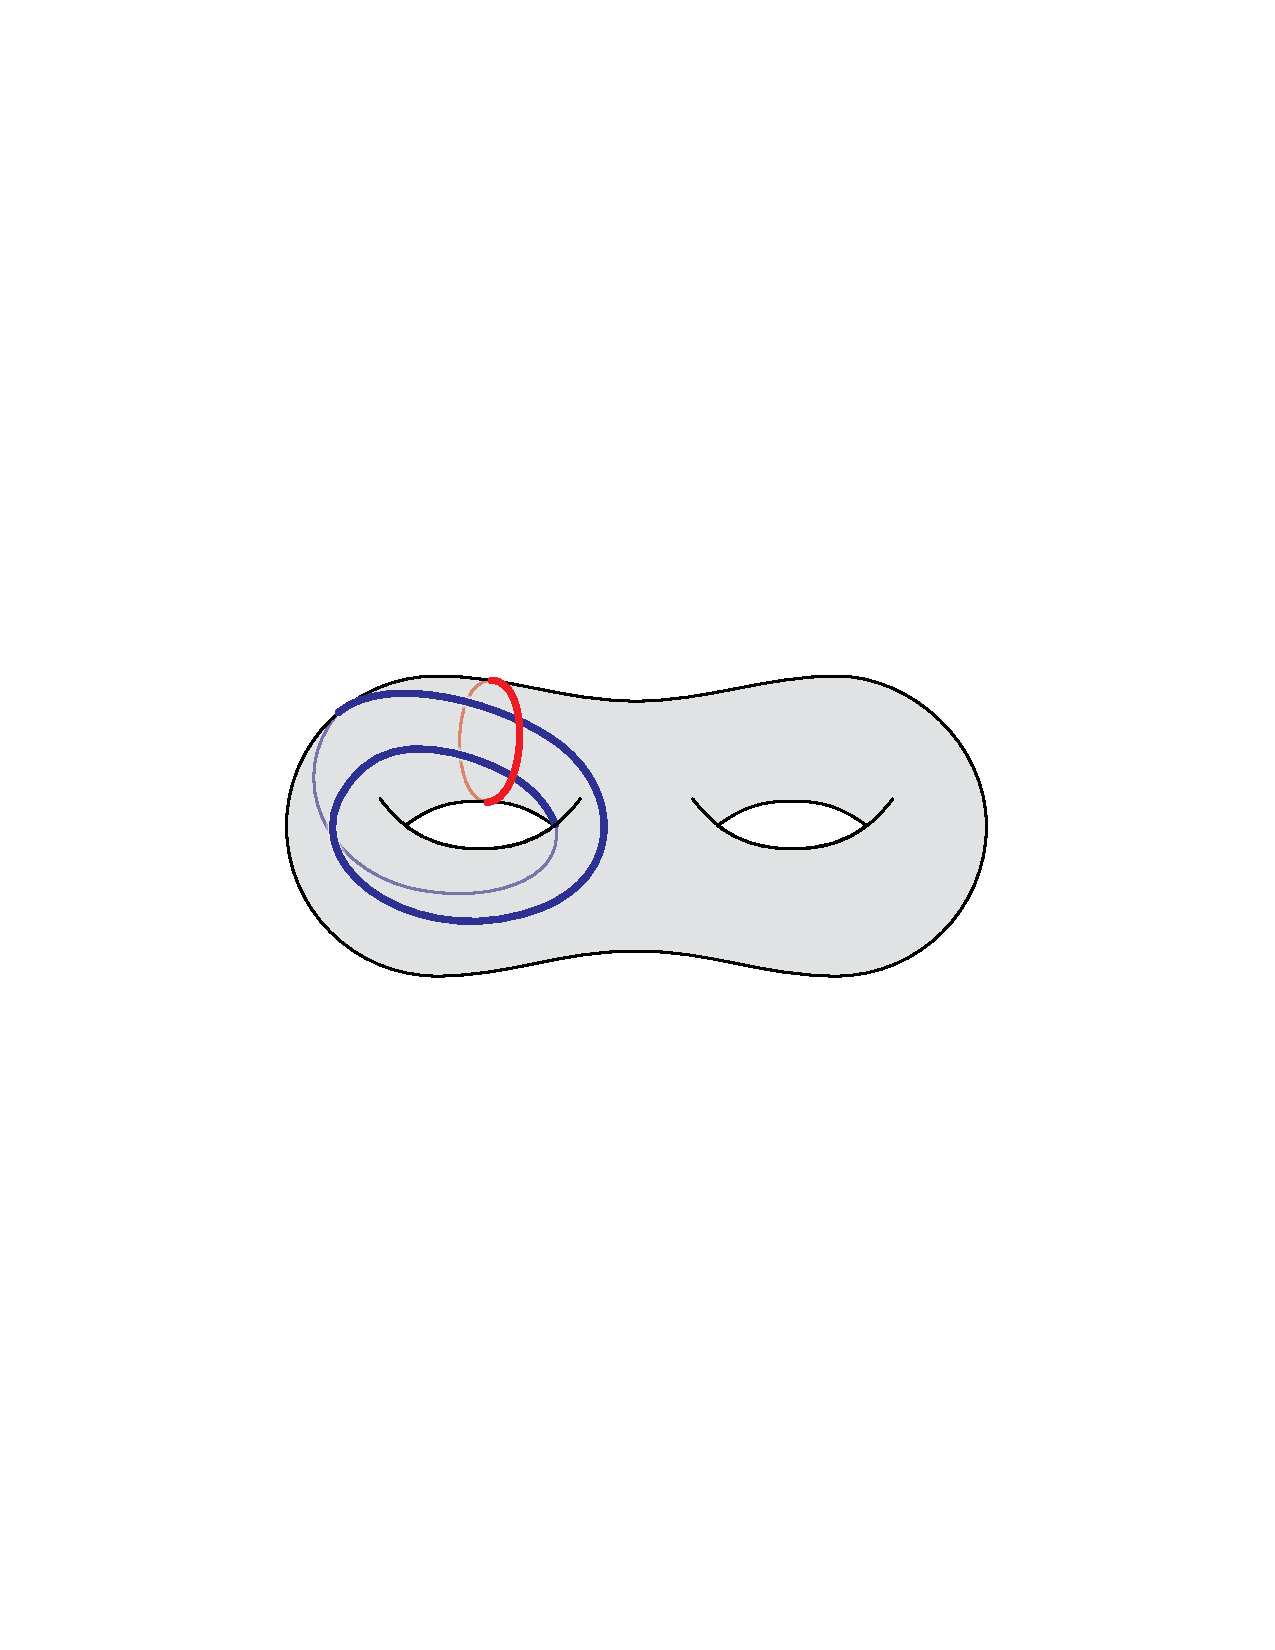
\includegraphics[height=0.75in]{Fig/homologous3}\\[2ex]
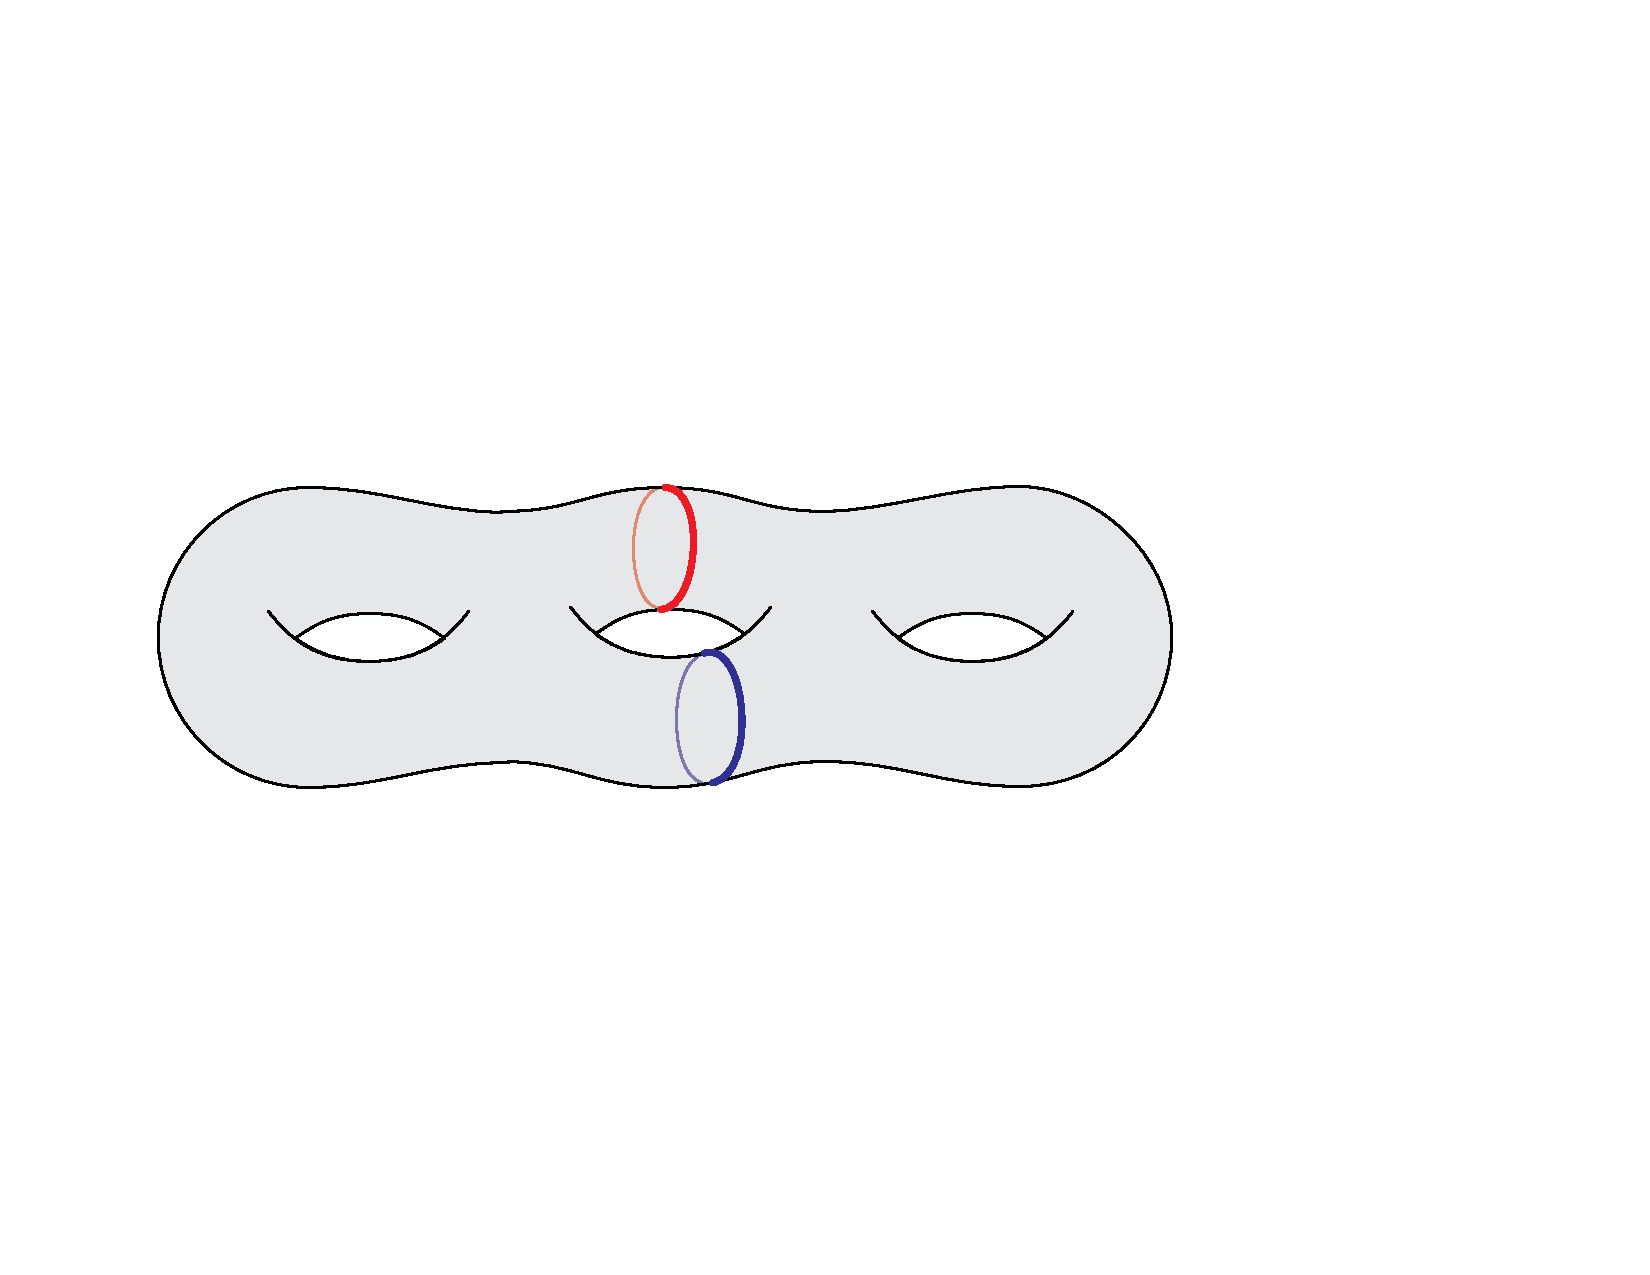
\includegraphics[height=0.75in]{Fig/homologous2}
\caption{Homologous pairs of cycles that are not homotopic.  (Lighter portions of the curves are on the back side of the surface.)}
\label{F:homology}
\end{figure}

\begin{figure}[htb]
\centering
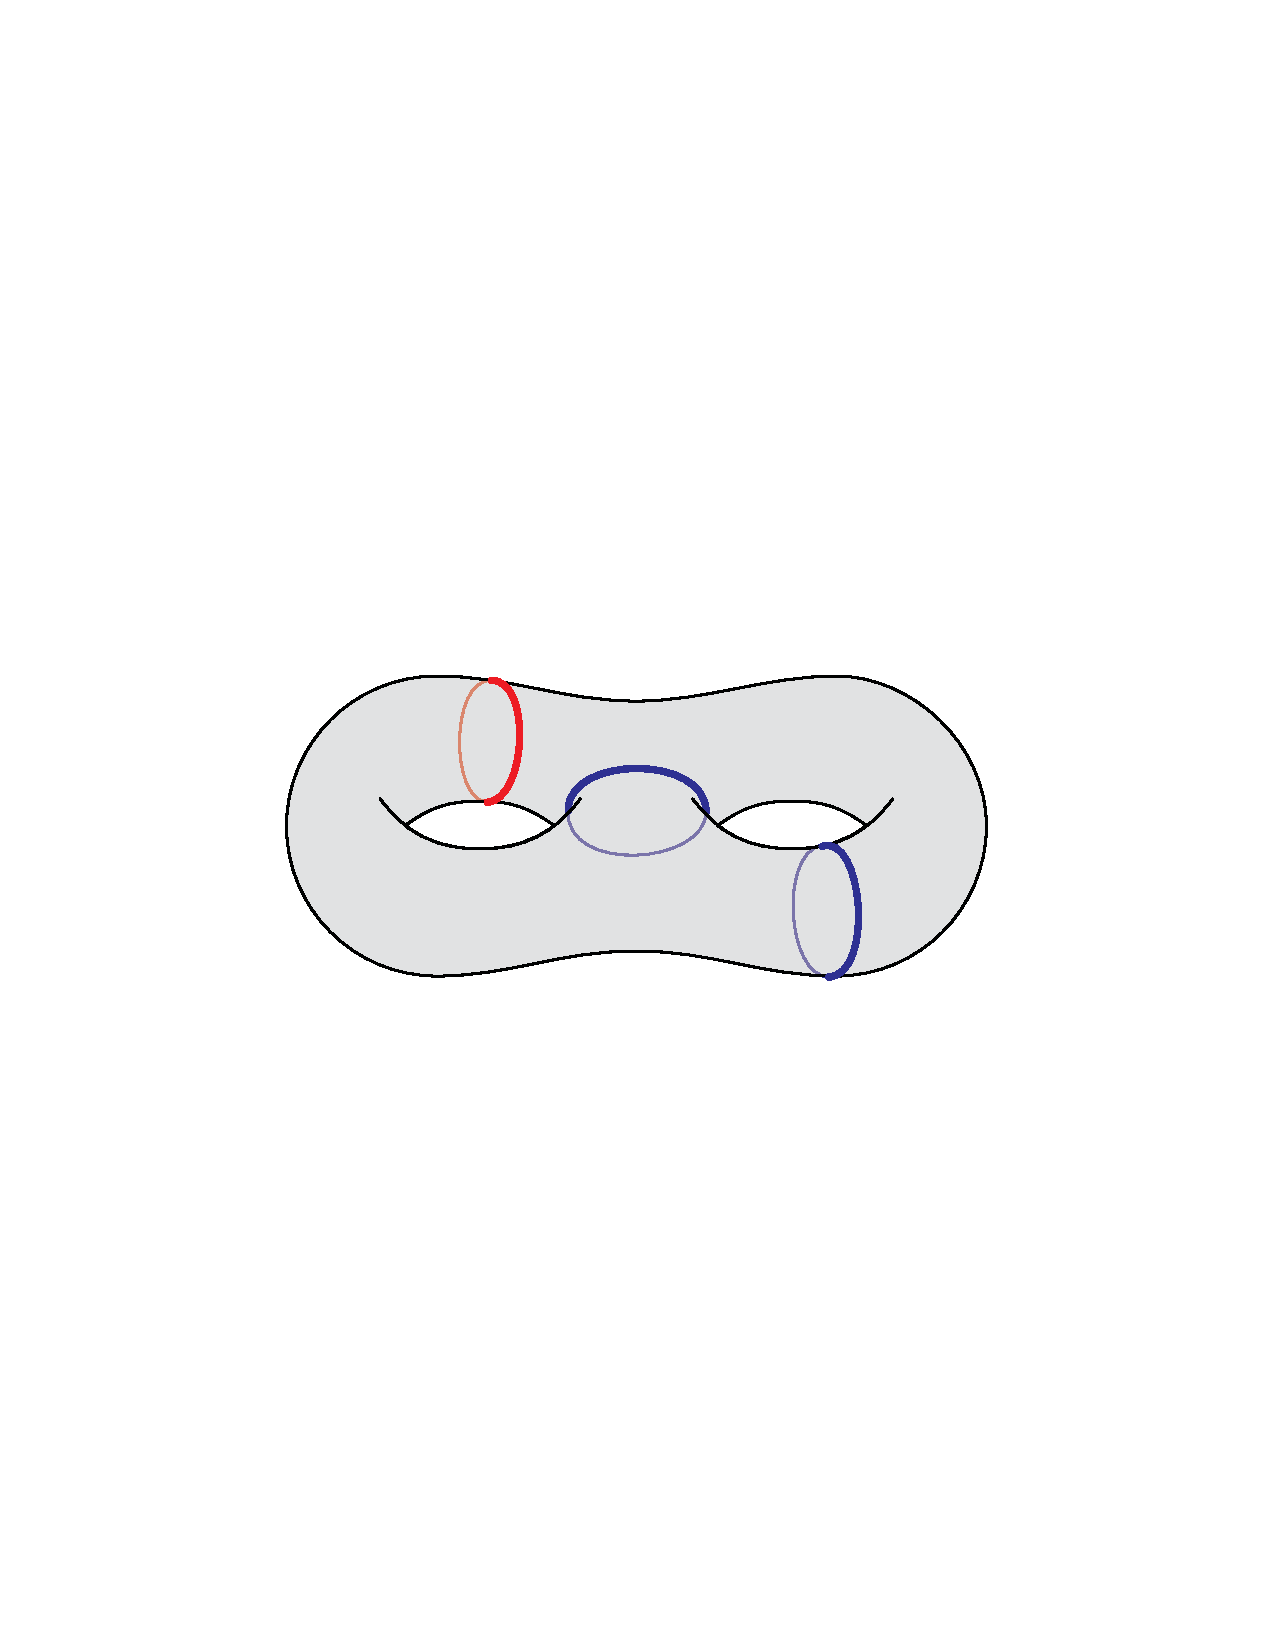
\includegraphics[height=0.75in]{Fig/homologous1}
\caption{Each cycle is homologous to the union of the other two.}
\label{F:homology2}
\end{figure}


%\begin{figure}[htb]
%\centering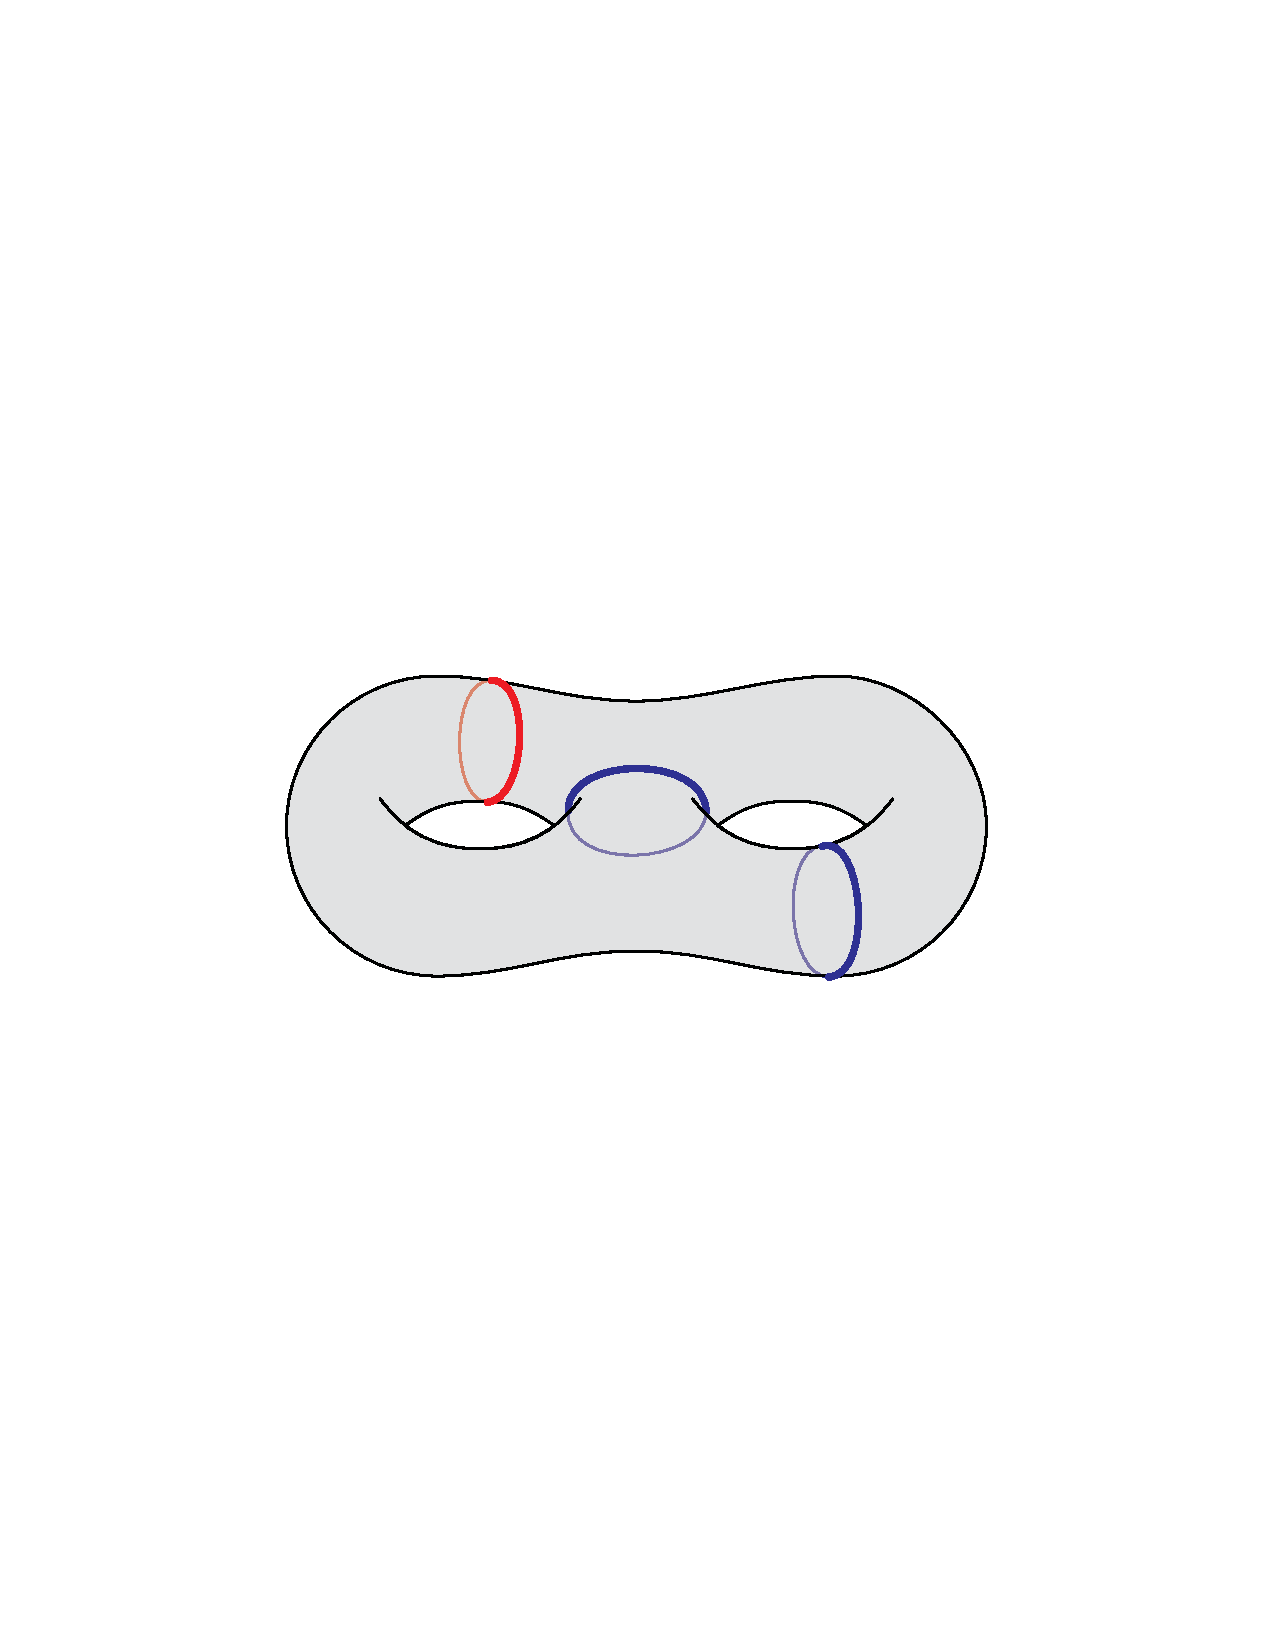
\includegraphics[height=1in]{Fig/homologous1}
%\caption{Each cycle is homologous with the union of the other two
%cycles.} \label{F:homology2}
%\end{figure}

The subgraphs of $G$ define a vector space isomorphic to $\Z_2^{\abs{E}}$, whose addition operation is symmetric difference, denoted $\oplus$.  Even subgraphs, boundary subgraphs, and homology classes all define subspaces of this vector space as follows.

The \EMPH{cycle space} $Z(G)$ is the vector space of all even subgraphs, which is (redundantly) generated by all cycles in $G$.  Every even subgraph satisfies $\abs{V}$ linear constraints, one at each vertex; however, exactly one of these constraints is redundant.  Thus, the cycle space is isomorphic to $\Z_2^{\abs{E}-\abs{V}+1}$.

The \EMPH{boundary space} $B(G)$ is the vector space of all boundary subgraphs, which is (redundantly) generated by the boundaries of faces of the embedding of $G$.  Any boundary subgraph is specified by a subset of the faces; a subset and its complement define the same boundary subgraph if and only if the surface has no boundary.  Thus $B(G)$ is isomorphic to $\Z_2^{\abs{F}-1}$ if $b=0$, and $\Z_2^{\abs{F}}$ if $b\ge 1$.   Because every boundary subgraph is even, $B(G)$ is a linear subspace of $Z(G)$. 

Finally, the \EMPH{homology space} $H(G)$ is the vector space of all homology classes of even subgraphs, which is isomorphic to $Z(G)/B(G)$.  Euler's formula implies that $H(G)$ has dimension $(\abs{E}-\abs{V}+1)-(\abs{F}-1) = 2g$ if $b=0$, or $(\abs{E}-\abs{V}+1)-\abs{F} = 2g+b-1$ if $b>0$.  In particular, any two graphs embedded on the same surface define isomorphic homology spaces, and the number of different homology classes is exactly $2^{2g+\max\set{0, b-1}}$.  The dimension $\beta = 2g+\max\set{0, b-1}$ of $H(G)$ is called the \emph{first Betti number} of the surface.

\subsection{Dual Graphs, Cocycles, and Cuts}

For any graph $G$ on a surface without boundary,\footnote{Graph duality can be generalized to surfaces with boundary \cite{ce-tspcs-06, ew-csec-08}, but this paper will not require such a generalization.} we can define a canonical \EMPH{dual graph $G^*$}.  The vertices of $G^*$ correspond to the faces of $G$, and two vertices in $G^*$ are are joined by a (dual) edge if and only if the corresponding faces of~$G$ are separated by an edge of $G$.  Thus, every edge~$e$ in~$G$ has a corresponding dual edge in $G^*$, denoted~\EMPH{$e^*$}.  For any face $f$ of~$G$, we let $f^*$ denote the corresponding vertex of $G^*$.  The dual graph $G^*$ has a cellular embedding on $\Sigma$, whose faces correspond exactly to the vertices of $G$.  For any vertex $v$ of~$G$, we let $v^*$ denote the corresponding face of $G^*$.  Duality is an involution---the dual of $G^*$ is isomorphic to the original graph~$G$.

\begin{figure}[htb]
\centering
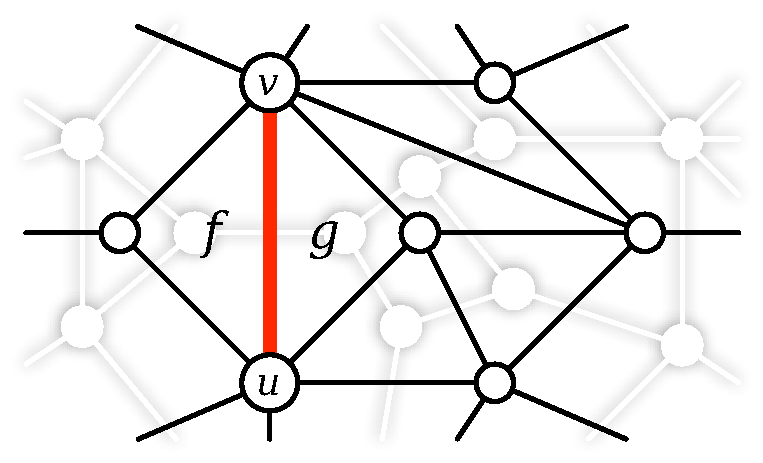
\includegraphics[height=0.9in]{Fig/primal}\quad
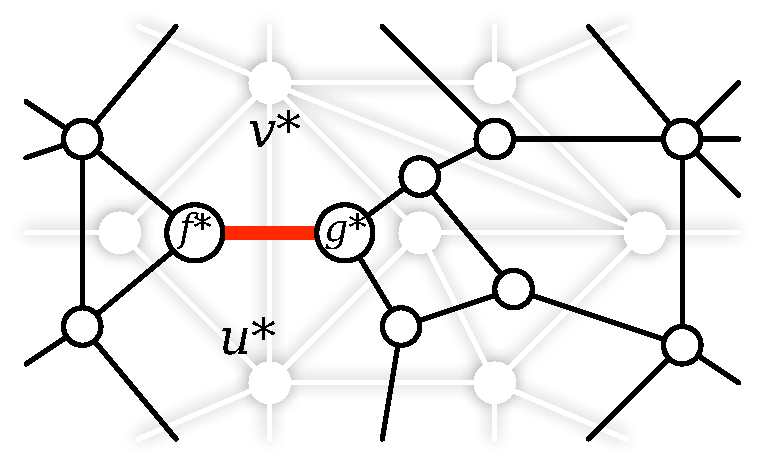
\includegraphics[height=0.9in]{Fig/dual}
\caption{Graph duality.  One edge $uv$ and its dual $(uv)^* =
f^*g^*$ are emphasized.} \label{F:primaldual}
\end{figure}

When the graph $G$ is fixed, we abuse notation by writing $H^*$ to denote the subgraph of $G^*$ containing the edges dual to the edges of a subgraph $H$ of $G$.  If a subgraph $H$ is a cycle, we call its dual $H^*$ a \EMPH{cocycle}; if a subgraph $H$ is a boundary subgraph, its dual $H^*$ is a \EMPH{cut}.  In planar graphs, every cocycle is a cut, and every minimal cut is a cocycle; however, these equivalences do not extend to higher-genus graphs.
% Two cocycles are \EMPH{cohomologous} if their symmetric difference is a cut, or equivalently, if their dual cycles are homologous.
%\note{Reviewer 2 says: "cohomologous is pedantic and never used later."}
%\note{Erin: Again, I disagree - I think the cohomologous should be included for completeness, and because it relates to dual cycles being homologous.}


% ----------------------------------------------------------------------------
\def\reverse#1{\smash{\overline{#1}}}

\section{Minimum Homologous Subgraphs}

Let $G$ be an $n$-vertex undirected graph, embedded on an orientable
surface with genus $g$ and $b$ boundary components, and let $H$
be an even subgraph of $G$.  In this section, we describe an
algorithm to compute the minimum-cost even subgraph homologous with
$H$ in $(g+b)^{O(g+b)}n\log n$ time.  In fact, our algorithm can be
modified easily to compute a minimum-cost representative in
\emph{every} homology class in the same asymptotic running time;
there are exactly $2^{2g+\max\set{b-1,0}}$ such classes.

Our algorithm closely resembles the algorithm of Chambers \etal~\cite{ccelw-scsih-08} for computing a shortest splitting cycle; in fact, our algorithm is somewhat simpler.  The first stage of our algorithm cuts the underlying combinatorial surface into a topological disk by a network of shortest paths.  Next, we enumerate all possible ways for an even subgraph to intersect each shortest path in the decomposition network $O(g+b)$ times.  We quickly discard any crossing pattern that does not correspond to an even subgraph in the desired homology class.  Each crossing pattern is realized by several \emph{homotopy} classes of sets of non-crossing cycles, which we easily enumerate.  Within each homotopy class, we find a minimum-length set of non-crossing cycles with each crossing pattern using an algorithm of Kutz \cite{k-csnco-06}.  The union of those cycles is an even subgraph in the desired homology class; we return the lightest such subgraph as our output.

To simplify the presentation of our results, we assume that there is a unique shortest path $\sigma(u,v)$ between any pair of vertices $u$ and $v$ in the input graph $G$.  If necessary, this assumption can be enforced (at least with high probability) using standard perturbation techniques \cite{mvv-memi-87}.

%\note{Reviewer 2 says: "before Section 3.1: Is it necessary to use the perturbation
%techniques, or do all your results work with minor changes without this
%assumption?"}

%\note{Erin: I think we need them here, because we often get into trouble without, but I haven't thought extensively about it.}

%\note{Jeff: I seriously doubt these matter.}

\subsection{Minimum Cuts}

Before we describe our algorithm, we first show that the minimum-weight homologous subgraph problem includes (the combinatorial dual of) the classical minimum-cut problem as a special case.

\begin{lemma}
Let $G=(V,E)$ be an edge-weighted graph embedded on a surface $\Sigma$ without boundary, and let $s$ and $t$ be vertices of~$G$.  Finally, let $X$ be the minimum-weight $(s,t)$-cut in~$G$.  Then~$X^*$ is the minimum-weight even subgraph of $G^*$ homologous with the boundary of $s^*$ in the surface $\Sigma\setminus(s^*\cup t^*)$.
\end{lemma}

\begin{proof}
Let $\partial s^*$ denote the boundary of $s^*$, and let $\Sigma'$ denote the surface $\Sigma\setminus {(s^*\cup t^*)}$.

Let $X$ be an arbitrary $(s,t)$-cut in $G$.  This cut partitions the vertices of $G$ into two disjoint subsets, $S$ and $T$, respectively containing vertices $s$ and $t$.  Thus, the dual subgraph $X^*$ partitions the faces of $G^*$ into two disjoint subsets, $S^*$ and $T^*$, respectively containing faces $s^*$ and $t^*$.  In particular, $X^*$ is the boundary of the union of the faces in $S^*$, which implies that $X^*$ is null-homologous in $\Sigma$.  The subgraph $X^* \oplus \partial s^*$ is the boundary of the union of $S^* \setminus\set{s^*}$, which is a subset of the faces of $\Sigma'$.  Thus,  $X^*\oplus \partial s^*$ is null-homologous in $\Sigma'$.  We conclude that $X^*$ and  $\partial s^*$ are homologous in $\Sigma'$.

Conversely, let $X^*$ be an arbitrary even subgraph of $G^*$ homologous to $\partial s^*$ in $\Sigma'$.  The subgraph $X^*\oplus \partial s^*$ is null-homologous in $\Sigma'$.  This immediately implies that $X^*$ is null-homologous in $\Sigma$; moreover, faces $s^*$ and $t^*$ are on opposite sides of $X^*$.   any path from $s$ to $t$ in the original graph $G$ must traverse at least one edge of $X$.  We conclude that $X$ is an $(s,t)$-cut.
\end{proof}

\subsection{Crossing Bound}

Our main technical lemma establishes an upper bound on the number of crossings between an arbitrary shortest path and the minimum-weight even subgraph in any homology class.  Crossing-number arguments were first used by Cabello and Mohar \cite{cm-fsnsn-07} to develop the first subquadratic algorithms for shortest non-contractible and non-separating cycles; their arguments are the foundation of all later improvements of their algorithm \cite{c-mdpg-06, k-csnco-06, cc-msspg-07}.  Our proof is quite similar to the argument of Chambers \etal~\cite{ccelw-scsih-08} that the shortest \emph{splitting} cycle crosses any shortest path $O(g+b)$ times.  However, our new proof is simpler, because the structure we seek is a true subgraph, which need not be connected, rather than a single (weakly) simple closed walk.

Stating our crossing bound is rather subtle, because we cannot consistently define when a shortest path crosses an even subgraph.  Instead, we partition the even subgraph into a well-behaved collection of cycles, and then consider the total number of crossings between a shortest path and the cycles in that collection.  Specifically, we define a \EMPH{cycle decomposition} of an even subgraph~$H$ to be a set of edge-disjoint, non-crossing, weakly simple cycles whose union is $H$.

\begin{lemma}
Every even subgraph of an embedded graph has a cycle decomposition.
\end{lemma}

\begin{proof}
Let $H$ be an even subgraph of $G$.  We can decompose $H$ into cycles by specifying, at each vertex $v$, which pairs of incident edges of $H$ are consecutive.  Any pairing that does not create a crossing at $v$ is sufficient.  For example, if $e_1, e_2, \dots, e_{2d}$ are the edges of $H$ incident to $v$, indexed in clockwise order around $v$, we could pair edges $e_{2i-1}$ and $e_{2i}$ for each $i$.  
\end{proof}

We emphasize that each cycle in a cycle decomposition may visit vertices multiple times; indeed, some even subgraphs cannot be decomposed into strictly simple cycles.

%\note{Reviewer 2 says: " In the proof of Lemma 3.2, an additional step is necessary: split every
%resulting cycle into simple ones."}

%\note{Erin: I think that our construction actually does this - the splitting is implied when we pick consecutive edges in clockwise order.  I don't think we should modify our proof here; it'll just confuse the issue.}


%
%  Unnecessary?  We need this for the time bound for each crossing pattern.
%
%\begin{lemma}
%If every edge of $G$ has positive weight, then the minimum-weight even subgraph in any $\Z_2$-homology class is the union of at most $g + \max\set{b-1,0}$ non-(self-)crossing cycles, each as short as possible in its individual homology class.
%\end{lemma}

%\begin{proof}
%Let $H$ be an even subgraph with minimum weight in its homology class, and suppose $H$ is the union of non-crossing simple cycles $\gamma_1, \dots, \gamma_r$.  No subset of these cycles is null-homologous; otherwise, removing that subset from $H$ would decrease its weight without changing its homology class.

%\note{blah$^3$}
%\end{proof}

%\note{Reviewer 2 says: Statement of Lemma 3.3: why not take an even subgraph instead of $\gamma_1$, ..., $\gamma_r$? Are these $\gamma_i$ edge-disjoint? "in its
%Z2-homology class": of what? "crosses $\gamma_1$,..., $\gamma_r$ at most
%... times": emphasize that it is the total number of crossings.}

%\note{Jeff: The crossing number of an even subgraph is not well-defined; it depends on the cycle decomposition.  The $\gamma_i$'s are edge-disjoint WLOG, but the lemma doesn't require that assumption.  ``\dots whose union is shortest in its homology class'' is unambiguous English.  Agree with emphasis.}

\begin{lemma}
\label{L:crossing}
Let $G$ be an edge-weighted graph embedded on a surface with genus $g$ and $b$ boundary components.  Let $H$ be a subgraph of $G$ of minimum weight in its $\Z_2$-homology class, and let $\gamma_1, \gamma_2, \dots, \gamma_r$ be a cycle decomposition of $H$.  The total number of crossings between any shortest path in $G$ and the cycles $\gamma_1, \gamma_2, \dots, \gamma_r$ is at most $6g+2b-3$.
\end{lemma}

\begin{proof}
Let $\sigma(y,z)$ denote the shortest path between any two vertices $y$ and~$z$, and let $\sigma = \sigma(u,v)$ for some vertices $u$ and~$v$.  Uniqueness of shortest paths implies that if $y$ and $z$ are vertices of $\sigma$, either the shortest path $\sigma(y,z)$ or its reversal $\sigma(z,y)$ is a subpath of $\sigma$.  Without loss of generality, we can assume that $\sigma$ crosses each cycle $\gamma_i$ at least once.  For each $i$, let~$x_i$ denote the number of times $\sigma$ and $\gamma_i$ cross, and let $x = x_1 + x_2 + \cdots + x_r$.  We need to prove that $x\le 6g+2b-3$.

Consider the graph $G/\sigma$ obtained from $G$ by contracting $\sigma$ to a single vertex $uv$.  This graph inherits a cellular embedding on $\Sigma$ from the cellular embedding of $G$.  Each cycle $\gamma_i$ is contracted to the union of $x_i$ simple non-crossing loops in $G/\sigma$ with basepoint $uv$.  Altogether, we obtain $x$ loops, which we denote $\ell_1, \ell_2, \dots, \ell_x$.

Suppose some loop $\ell_i$ is contractible.  This loop is the contraction of a path $\pi_i$ in $G$ whose endpoints~$u_i$ and $v_i$ lie in $\sigma$.  The cycle $\delta = \pi_i \cdot \sigma(v_i,u_i)$ is also contractible.  Thus, the even subgraph $H\oplus\delta$ is homologous with $H$.  Moreover, the uniqueness of shortest paths implies that the weight of $H\oplus\delta = H \cup \sigma(v_i,u_i) \setminus \pi_i$ is smaller than the weight of~$H$.  But this contradicts our assumption that $H $ has minimum weight in its homology class.

Now suppose some pair of loops $\ell_i$ and $\ell_j$ are homotopic; by definition, the cycle $\ell_i\cdot\reverse{\ell_j}$ is contractible.  These two loops are contractions of paths $\pi_i$ and $\pi_j$ in $G$ with endpoints in $\sigma$.  Let $u_i$ and~$v_i$ denote the endpoints of $\pi_i$, and let $u_j$ and~$v_j$ denote the endpoints of $\pi_j$.  The cycle $\pi_i \cdot \sigma(v_i,v_j) \cdot \overline{\pi_j} \cdot \sigma(u_j, u_i)$ in $G$ is also contractible.  Let $\delta$ denote the set of edges of $G$ that appear in this cycle exactly once.  If the sub-paths $\sigma(v_i,v_j)$ and $\sigma(u_j, u_i)$ are edge-disjoint, then $\delta$ is a contractible cycle; otherwise, $\delta$ is the union of two non-crossing homotopic cycles.  In either case, $\delta$ is a boundary subgraph, so the symmetric difference $H\oplus\delta$ is homologous with $H$.  Moreover, $H\oplus\delta$ has smaller weight than~$H$, and we obtain another contradiction.

We conclude that the loops $\ell_1, \ell_2, \dots, \ell_x$ lie in distinct nontrivial homotopy classes.  Thus, these loops define an embedding of a single-vertex graph with $x$ edges onto $\Sigma$, where no face of the embedding is a disk bounded by less than three edges.  Euler's formula now implies that $x\le 6g+2b-3$~\cite[Lemma~2.1]{ccelw-scsih-08}.
\end{proof}

We emphasize that different cycle decompositions of the same even subgraph may lead to different numbers of crossings.  Our crossing bound applies to \emph{any} cycle decomposition.

\subsection{Systems of Paths and Crossing Vectors}

We are now ready to describe our algorithm.  The input consists of an edge-weighted graph $G$, embedded on a surface $\Sigma$ with genus~$g$ and $b$ boundary components, along with an even subgraph $H$ of $G$.  Our algorithm computes the minimum-weight even subgraph of $G$ that is homologous with $H$.

Our algorithm begins by computing a set $P$ of paths, each of which is the concatenation of two shortest paths (possibly meeting in the interior of an edge), such that the surface $\Sigma\setminus P$ is a topological disk.  If the $\Sigma$ has no boundary, the paths in $P$ are non-contractible loops with an arbitrary common basepoint; Euler's formula implies that the number of loops is $2g$.  Specifically, we construct a \emph{greedy system of loops} in $O(n\log n + gn)$ time, using an algorithm of Erickson and Whittlesey \cite{ew-gohhg-05}.  If the surface has boundary, the paths in $P$ are non-contractible arcs; Euler's formula implies that the number of arcs is $2g+b-1$.  Specifically, we again construct a \emph{greedy system of arcs} in $O(n\log n + (b+g)n)$ time, using a modification of Erickson and Whittlesey's algorithm described by Chambers \etal~\cite{ccelw-scsih-08}.

Let $p_1, p_2, \dots, p_\beta$ denote the paths in $P$, where $\beta = 2g + \max\set{0,b-1}$.  It is no coincidence that the number of paths in $P$ is equal to the dimension of the homology group $H(G)$.  Indeed, we can identify the homology class of any even subgraph by considering the number of times it crosses each path in $P$, as follows.

For any cycle $\gamma$ and any index $i$, let $x_i(\gamma)$ denote the number of times $\gamma$ crosses the path~$p_i$.  The \emph{crossing vector} $x(\gamma)$ is the vector $(x_1(\gamma), \dots, x_\beta(\gamma))$.  The crossing vector of a set of cycles is the sum of the crossing vectors of its elements.  Crossing vectors are not well-defined for arbitrary even subgraphs; different cycle decompositions can yield different crossing numbers.  However, the \emph{parity} of the crossing numbers is independent of the cycle decomposition.  The \emph{crossing parity vector} of any even subgraph $H$ is the bit vector $\bar{x}(H) = (\bar{x}_1, \dots, \bar{x}_\beta)$, where $\bar{x}_i = 1$ if the path $p_i$ crosses (any cycle decomposition of) $H$ an odd number of times, and $x_i = 0$ otherwise.

\begin{lemma}
Two even subgraphs are homologous if and only if their crossing parity vectors are equal.
\end{lemma}

\begin{proof}
Every boundary subgraph is the symmetric difference of facial cycles.  Any non-contractible loop or arc crosses facial cycle an even number of times; thus, the crossing parity vector of any facial cycle is the zero vector.  Every pair of even subgraphs $H$ and $H'$ satisfies the identity $x(H\oplus H') = x(H) \oplus x(H')$.  Thus, the crossing parity vector of any boundary subgraph is the zero vector.
\end{proof}

\begin{lemma}
We can compute the crossing parity vector of any even subgraph in $O(gn)$ time.
\end{lemma}

\begin{proof}
We can compute a cycle decomposition $\gamma_1, \dots, \gamma_r$ of $H$ in $O(n)$ time, by following the proof of Lemma \ref{L:crossing}.  We can compute the number of crossings between any cycle $\gamma_i$ and any path $p_j$ in time proportional to the number of edges in $\gamma_i$.  Thus, we can compute each bit $\bar{x}_j(H)$ in $O(n)$ time.
\end{proof}

We call an integer vector $(x_1, \dots, x_\beta)$ a \emph{valid
crossing vector} if $x_i \le 12g+4b-6$ for all $i$ and $({x_1\bmod
2}, \dots,\allowbreak {x_\beta\bmod 2}) = \bar{x}(H)$.  Our
algorithm enumerates all $(g+b)^{O(g+b)}$ valid crossing vectors by
brute force in ${(g+b)}^{O(g+b)}$ time.  Then for each valid
crossing vector, our algorithm computes the minimum-weight
collection of cycles with that crossing vector, as we describe next.

\subsection{Triangulations and Crossing Sequences}

We can cut our combinatorial surface $\Sigma\setminus P$ into a $2\beta$-gon, or \emph{abstract polygonal schema}, by cutting along each path in $P$ and replacing each copy of each path in the cut surface with a single edge.  Thus, each path in $P$ corresponds to two edges of this polygon. The vertices correspond to copies of the common basepoint of $P$ if $\Sigma$ has no boundary, or to boundary paths between endpoints of $P$ otherwise.

We dualize the abstract polygonal schema by replacing each edge with a vertex, and connecting vertices which correspond to adjacent edges in the primal schema.  Any collection of non-crossing, non-self-crossing cycles corresponds to a \emph{weighted triangulation} \cite{ccelw-scsih-08}, where we draw an edge between two vertices of the dual abstract polygonal schema if and only if some cycle consecutively crosses the corresponding pair of paths in the greedy system of loops.  Each edge is weighted by the number of times such a crossing occurs in our collection.  Conversely, a weighted triangulation corresponds to a collection of non-crossing, non-self-crossing cycles as long as corresponding vertices are incident to edges of equal total weight.  Lemma~\ref{L:crossing} implies that we only need to consider weights between 0 and $O(g+b)$.  Thus, there are $(g+b)^{O(g+b)}$ different weighted triangulations for each valid crossing vector.


\begin{figure}[htb]
\centering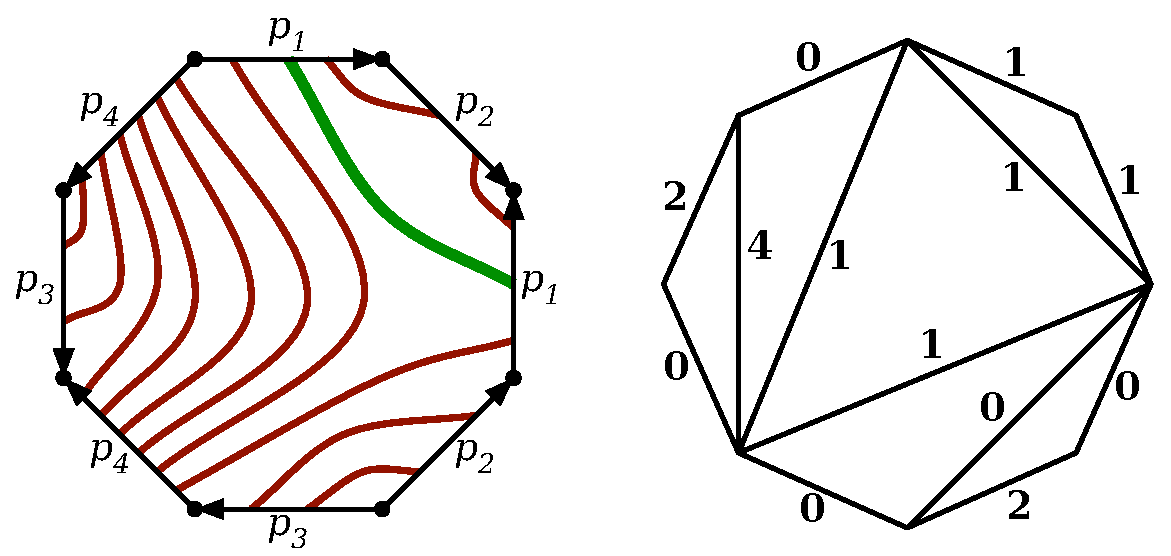
\includegraphics[height=1.45in]{Fig/triangulation}
\caption{Two disjoint simple cycles on a surface of genus 2, and the corresponding weighted triangulation.}
\end{figure}

For each valid weighted triangulation, we can compute a corresponding collection of abstract cycles in $O((g+b)^2)$ time by brute force.  In the same time, we can also compute the \emph{sequence} of crossings of each abstract cycle with the paths in $P$.  An algorithm of Kutz~\cite{k-csnco-06} computes the shortest cycle in $G$ with a given crossing sequence of length $x$ in $O(x n \log n)$ time, by gluing together $x$ copies of the planar surface $\Sigma\setminus P$ into an annulus and calling Frederickson's planar minimum-cut algorithm \cite{f-faspp-87}.  Thus, for each weighted triangulation, we obtain the shortest corresponding set of cycles in $O((g+b)^2 n \log n)$ time.

%\note{Can't we almost directly steal the figures from the splitting
%paper, but modify them to be a collection of loops instead of a
%single cycle?  Jeff, I don't have copies of those ai files - do you?
%We could include them in a revision, if not the first submission.}

%
%Suppose $\gamma_1, \gamma_2, \dots, \gamma_r$ are simple
%non-crossing cycles whose union is the shortest even subgraph
%homologous with $H$.  Lemma \ref{L:crossing} implies that these
%cycles are modeled by $O((g+b)^2)$ segments in the abstract
%polygonal schema, so the virtual crossing numbers for these cycles
%sum to $O((g+b)^3)$.
%
%For each valid crossing vector $x = (x_1, \dots, x_\beta)$, our
%algorithm enumerates the set of $(g+b)^{O(g+b)}$ virtual crossing
%vectors that are consistent with $x$ in $(g+b)^{O(g+b)}$ time.  For
%each virtual crossing vector, we construct the corresponding set of
%abstract cycles in $O((g+b)^3)$ time; each abstract cycle has
%complexity $O((g+b)^2)$.  Using an algorithm of Kutz
%\cite{k-csnco-06}, we compute the shortest cycle in $G$ with the
%same crossing \emph{sequence} as each abstract cycle.  We report the
%union of those cycles as the minimum-weight even subgraph consistent
%with that virtual crossing vector.
%


\begin{theorem}
Let $G$ be a graph with positively weighted edges embedded on a surface with genus
$g$ and $b$ boundary components, and let $H$ be an even subgraph of $G$.
We can compute the minimum-cost even subgraph homologous with $H$ in
$(g+b)^{O(g+b)} n\log n$ time.
\end{theorem}

\begin{corollary}
Let $G$ be an edge-weighted graph embedded on a surface with genus $g$ and $b$ boundary components, and let $s$ and $t$ be vertices of $G$.  We can compute the minimum-weight $(s,t)$-cut in $G$ in $g^{O(g)} n\log n$ time.
\end{corollary}



% ----------------------------------------------------------------------------
\section{{NP}-hardness}
\label{S:NP-hard}

In this section, we show that finding the minimum-weight even subgraph in a given homology class is {NP}-hard, even when the underlying surface has no boundary.

Chen and Freedman \cite{cf-qhc-08, cf-qhc2-07} proved a similar hardness result (by reduction from a special case of \textsc{Max2Sat}) for general simplicial complexes; however, the complexes output by their reduction are never manifolds.  Chambers \etal~\cite{ccelw-scsih-08} prove that finding the shortest \emph{splitting} cycle is {NP}-hard; a cycle is splitting if it is non-self-crossing, non-contractible, and null-homologous.  A simple modification of their reduction (from Hamiltonian cycle in planar grid graphs) implies that finding the shortest \emph{strictly simple cycle} in a given homology class is {NP}-hard.  Our proof closely follows a reduction of McCormick \etal~\cite{mrr-edofm-03} from \textsc{Min2Sat} to a special case of \textsc{MaxCut}.

\begin{theorem}
Computing the minimum-cost even subgraph in a given homology class on a surface without boundary is equivalent to computing a minimum-capacity cut in an embedded edge-weighted graph $G$ whose negative-cost edges are dual to an even subgraph in $G^*$.
\end{theorem}

\begin{proof}
Fix a graph $G$ embedded on a surface $\Sigma$ without boundary, together with a cost function $c\colon E\to \Real$.  For any even subgraph $H$ of $G$, let $c(H) = \sum_{e\in H} c(e)$, and let $\textsc{MinHom}(H,c)$ denote the even subgraph of minimum cost in the homology class of $H$.

Consider the \emph{residual cost} function $c_H\colon E\to \Real$ defined by setting $c_H(e) = c(e)$ for each edge $e\not\in H$, and $c_H(e) = -c(e)$ for each edge $e\in H$.  For any subgraph $H'$ of $G$, we have $c(H') = c_H(H\oplus H') + c(H)$, which immediately implies that
\(
    \textsc{MinHom}(H,c) ~=~
    H \oplus \textsc{MinHom}(\varnothing, c_H).
\)

Every null-homologous even subgraph of $G$ is dual to a cut in the dual graph $G^*$.  Thus, we have reduced our problem to computing the minimum cut in $G^*$ with respect to the cost function $c_H$.  Since the empty set is a valid cut with zero cost, the cost of the minimum cut is never positive.  In particular, $H$ is the minimum-cost even subgraph in its homology class if and only if the cut in $G^*$ with minimum residual cost is empty.

In fact, our reduction is reversible.  Suppose we want to find the minimum cut in an embedded graph $G = (V, E)$ with respect to the cost function $c\colon E\to \Real$, where every face of $G$ is incident to an even number of edges with negative cost.  Let $H = \set{{e\in E}\mid {c(e)<0}}$ be the subgraph of negative-cost edges, and let $X$ denote the (possibly empty) set of edges in the minimum cut of $G$.  Consider the \emph{absolute cost} function $\abs{c}\colon E^*\to \Real$ defined as $\abs{c}(e^*) = \abs{c(e)}$.  Then $(H\oplus X)^*$ is the even subgraph of $G^*$ of minimum absolute cost that is homologous to $H^*$.
\end{proof}

We now prove that this special case of the minimum cut problem is {NP}-hard, by  reduction from \textsc{MinCut} in graphs with negative edges.  This problem includes \textsc{MaxCut} as a special case (when every edge has negative cost), but many other special cases are also {NP}-hard~\cite{mrr-edofm-03}.  The output of our reduction is a simple triangulation; the reduction can be simplified if graphs with loops and parallel edges are allowed.

Suppose we are given an \emph{arbitrary} graph $G = (V,E)$ with $n$ vertices and an \emph{arbitrary} cost function $c\colon E\to \Real$.  We begin by computing a cellular embedding of $G$ on some surface.  If we don't care whether the surface is orientable, we can simply impose a cyclic order on the edges incident to each vertex.  The maximum-genus \emph{orientable} cellular embedding can be computed in polynomial time~\cite{fgm-fmggi-88}.  Alternately, we can add zero-length edges to make the graph complete and then use classical results of Ringel, Youngs, and others \cite{ry-shmcp-68,r-mct-74} to compute a minimum-genus orientable embedding of $K_n$ in polynomial time.  Once we have an embedding, we add vertices and zero-cost edges to obtain a triangulation.

Let $C$ be the sum of the absolute values of the edge costs: $C:= \sum_e \abs{c(e)}$.  We locally modify both the surface and the embedding to transform each negative-weight edge into a cocycle, as follows.  We transform the edges one at a time; after each iteration, the embedding is a simple triangulation.  (Our reduction can be simplified if a simple graph is not required.)  For each edge~$uv$ with $c(uv)<0$, remove $uv$ to create a quadrilateral face.  Triangulate this face as shown in Figure \ref{F:addhandle}; we call the new faces $uu_1u_2$ and $vv_1v_2$ \emph{endpoint triangles}.  Assign cost $C$ to the edges of the endpoint triangles and cost zero to the other new edges. Glue a new handle to the endpoint triangles, and triangulate the handle with a cycle of six edges, each with cost $c(uv)/6$.  These six edges form a cocycle of cost $c(uv)$, which we call an \emph{edge cocycle}, in the new embedding.  Each iteration adds $5$ vertices and $21$ edges to the graph and increases the genus of the underlying surface by $1$.

\begin{figure}[hbt]
\centering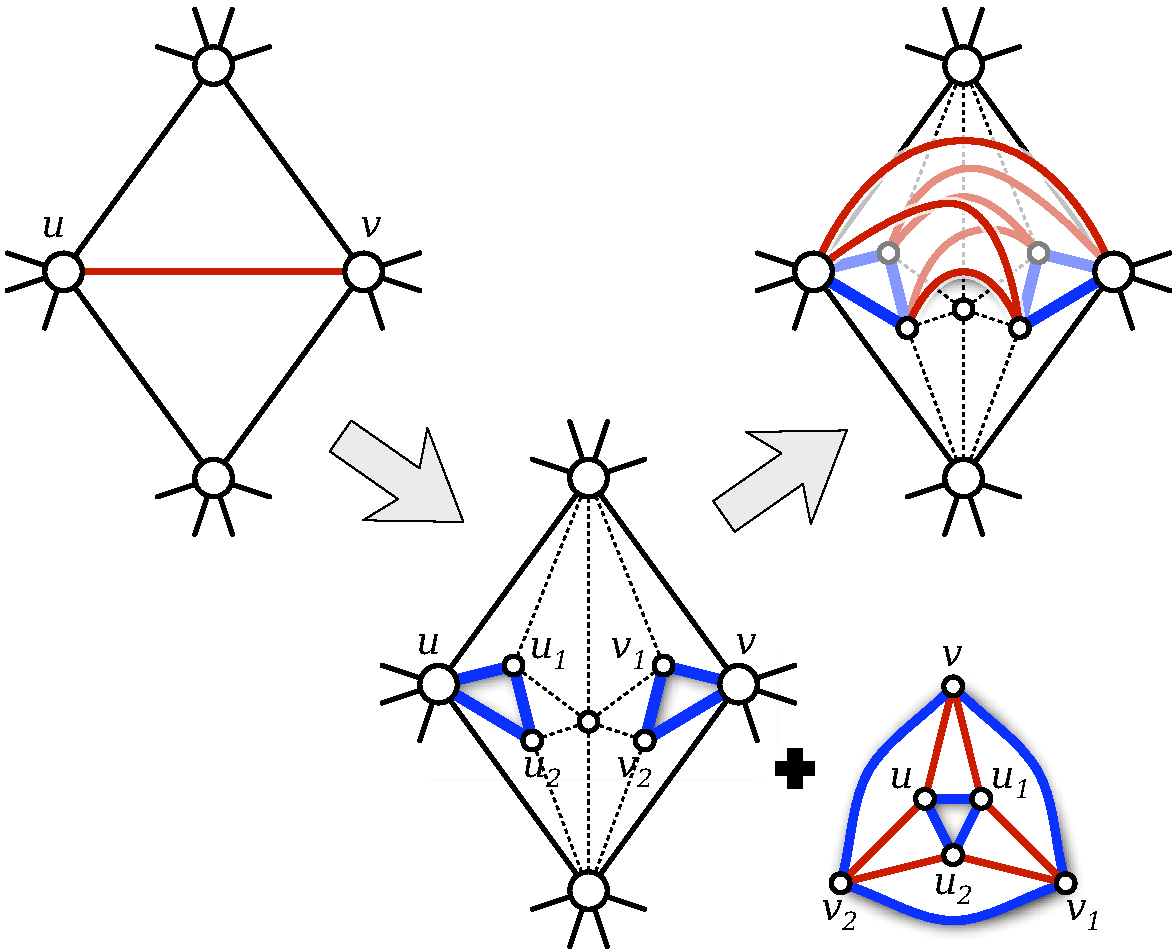
\includegraphics[height=2.25in]{Fig/addhandle3}
\caption{Adding a handle to transform a negative edge into a negative cocycle.  Thick (blue) edges have cost $C$; dashed edges have cost zero.}
\label{F:addhandle}
\end{figure}

Let $G'$ denote the transformed graph and $c'\colon E(G')\to \Real$ its associated cost function.  The minimum cut in $G'$ cannot contain any edge of an endpoint triangle.  Thus, for each edge cocycle, either all six edges cross the cut, or none of them cross the cut.  It follows that the minimum cut in $G'$ corresponds to a cut with equal cost in the original graph $G$.  Conversely, any cut in $G$ can be transformed into a cut in~$G'$ of equal cost.  Thus, computing the minimum cut in $G'$ is equivalent to computing the minimum cut in $G$.

\begin{theorem}
Given an even subgraph $H$ of an edge-weighted graph $G$ embedded on a surface without boundary, computing the minimum-weight even subgraph homologous to $H$ is strongly {NP}-hard.
\end{theorem}

Our reduction can be modified further to impose other desirable properties on the output instances, for example, that the graph is unweighted, every vertex has degree $3$, or the input subgraph $H$ is a simple cycle.  We leave the details as easy exercises for the reader.

%Interestingly, any instance built by our reduction can be further reduced to $3^g$ instances of minimum $(s,t)$-cut in a graph of genus $O(g)$.  For each edge cocycle, we guess which sides of the cut contains its vertex triangles.  If they lie on different sides, we remove the handle, join the vertices on one vertex triangle to a common supersource~$s$, and join the vertices of the other vertex triangle to a common supersink~$t$.  (If they lie on the same side, we do nothing to the cocycle.)  After modifying the graph, we compute the minimum-cost $(s,t)$-cut.

Finally, we emphasize that the {NP}-hardness of this problem relies crucially on the fact that we are using homology with coefficients taken from the finite field $\Z_2$.  The corresponding problem for homology with real or integer coefficients is a minimum-cost circulation problem, and thus can be solved in polynomial time.  In our companion paper \cite{cen-hfcc-09}, we show that this circulation problem can be solved in near-linear time for graphs of constant genus, using very different techniques.


% ----------------------------------------------------------------------
\section{Conclusions and Open Problems}

Many potential improvements and open questions remain.  For example, unlike the flow algorithms described in our companion paper \cite{cen-hfcc-09}, our minimum-cut algorithm does not seem to extend easily to embedded \emph{directed} graphs.  Computing minimum cuts in directed graphs embedded on a surface in near-linear time remains an open question.

We conjecture that both maximum flows and minimum cuts in embedded graphs can be computed in $O(g^k n\log n)$ time for some small constant $k$, perhaps using a
generalization of the network simplex algorithm of Borradaile and
Klein \cite{b-epnfc-08, bk-tamfd-06, bk-amfdp-09}.  Even the special
case of unit capacities is open.

It seems likely that our minimum-cut algorithm will extend to graphs embedded on non-orientable surfaces; the main challenge is extending Lemma \ref{L:crossing}.  (In contrast, our techniques for computing maximum flows will not extend to non-orientable surfaces without substantial modification, in part because our definition of duality for directed graphs requires a consistent surface orientation.)  No near-linear-time algorithms are known in this setting, even for graphs embedded on the projective plane.

\paragraph{Acknowledgments}
The authors would like to thank Chandra Chekuri and Aparna Sundar for helpful discussions, and the anonymous reviewers for their comments and suggestions.

%\nocite{*}
\bibliographystyle{newabuser}
\bibliography{topology,optimization,data-structures}

\end{document}
